\documentclass[aspectratio=169,11pt]{beamer}

\usepackage[T1]{fontenc}
\usepackage{lmodern}
\usepackage{amsmath,amssymb,bm}
\usepackage{tikz}
\usepackage{listings}
\usepackage{graphicx}
\usetikzlibrary{arrows.meta,positioning,calc,fit,shapes.geometric}

% ---------- Visual system ----------
\definecolor{VBlue}{HTML}{173B63}
\definecolor{VCyan}{HTML}{18A6A6}
\definecolor{VGold}{HTML}{F2A33A}
\definecolor{VInk}{HTML}{182431}
\definecolor{VMuted}{HTML}{667482}
\definecolor{VLight}{HTML}{EFF4F6}
\definecolor{VLine}{HTML}{D7E2E7}
\definecolor{VWhite}{HTML}{FFFFFF}

\setbeamercolor{normal text}{fg=VInk,bg=VWhite}
\setbeamercolor{frametitle}{fg=VBlue,bg=VWhite}
\setbeamertemplate{navigation symbols}{}
\setbeamersize{text margin left=0.78cm,text margin right=0.78cm}

\setbeamerfont{frametitle}{size=\Large,series=\bfseries}
\setbeamertemplate{frametitle}{%
  \vspace{0.08cm}
  \begin{beamercolorbox}[wd=\textwidth,sep=0pt]{frametitle}
    \insertframetitle
  \end{beamercolorbox}
  \vspace{0.08cm}\color{VCyan}\rule{\textwidth}{0.65pt}
}

% Code snippet styling
\lstdefinestyle{mystyle}{
    backgroundcolor=\color{VLight},   
    commentstyle=\color{VCyan},
    keywordstyle=\color{VBlue}\bfseries,
    numberstyle=\tiny\color{VMuted},
    stringstyle=\color{VGold},
    basicstyle=\ttfamily\scriptsize,
    breakatwhitespace=false,         
    breaklines=true,                 
    captionpos=b,                    
    keepspaces=true,                 
    numbers=none,                    
    showspaces=false,                
    showstringspaces=false,
    showtabs=false,                  
    tabsize=2,
    frame=single,
    rulecolor=\color{VLine}
}
\lstset{style=mystyle, language=Python}

\begin{document}

% -----------------------------------------------------------------------------
\begin{frame}[plain]
  \begin{tikzpicture}[remember picture,overlay]
    \fill[VBlue] (current page.south west) rectangle (current page.north east);
    \fill[VCyan] (current page.south west) rectangle ([xshift=0.20cm]current page.north west);
    
    \node[anchor=west,text=white,font=\fontsize{44}{46}\selectfont\bfseries]
      at ([xshift=1.05cm,yshift=0.55cm]current page.west) {VOOGLE};
    \node[anchor=west,text=VCyan,font=\fontsize{20}{24}\selectfont\bfseries]
      at ([xshift=1.08cm,yshift=-0.48cm]current page.west)
      {Audio Intelligence Through Hard Mathematics};
    \node[anchor=west,text=white!72,font=\large]
      at ([xshift=1.10cm,yshift=-1.22cm]current page.west)
      {DSP \enspace$\rightarrow$\enspace Feature Extraction \enspace$\rightarrow$\enspace Metric Search};
  \end{tikzpicture}
\end{frame}

% -----------------------------------------------------------------------------
\begin{frame}[fragile,t]{Philosophy \& Motivation}
  \vspace{0.3cm}
  
  \textbf{The Problem:} Modern audio AI (Neural Networks) is a "black box" that requires massive GPU compute and hides the physical properties of sound.
  
  \vspace{0.4cm}
  \textbf{The Voogle Solution:}
  \begin{itemize}
      \item \textbf{Deterministic Math:} 100\% classical signal processing.
      \item \textbf{Physical Grounding:} We measure actual vocal tract resonance, kinetic energy, and spectral geometry.
      \item \textbf{High Efficiency:} Sub-second retrieval using $O(1)$ Hash Inverted Indexes and $O(\log n)$ KD-Trees.
  \end{itemize}
  
  \vspace{0.4cm}
  \textit{"Can we build a complete audio search engine using only pure mathematics?"}
\end{frame}

% -----------------------------------------------------------------------------
\begin{frame}[fragile,t]{System Architecture}
  \vspace{0.2cm}
  
  \centering
  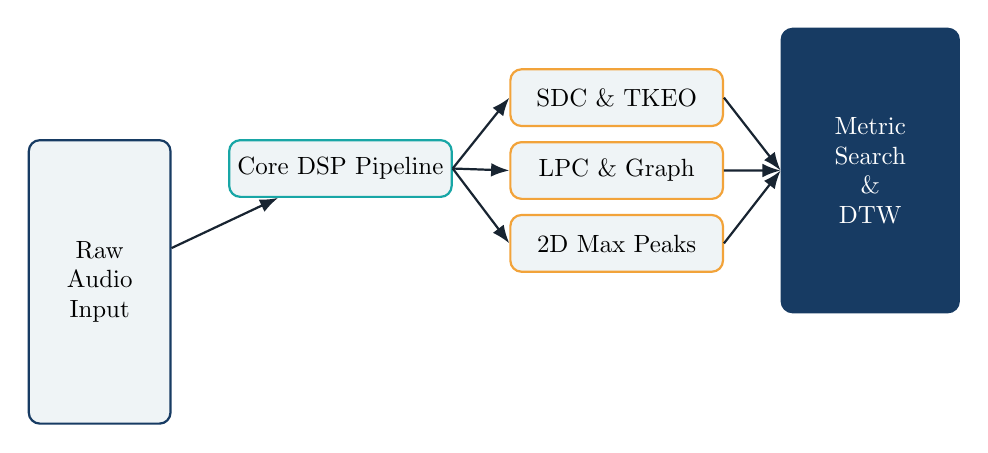
\begin{tikzpicture}[node distance=0.8cm,>=Latex,scale=0.9,transform shape]
    \node[draw=VBlue,thick,fill=VLight,rounded corners,align=center,minimum width=2cm,minimum height=4cm] (input) {Raw\\Audio\\Input};
    
    \node[draw=VCyan,thick,fill=VLight,rounded corners,align=center,minimum width=3cm,minimum height=0.8cm, right=of input, yshift=1.6cm] (dsp) {Core DSP Pipeline};
    
    \node[draw=VGold,thick,fill=VLight,rounded corners,align=center,minimum width=3cm,minimum height=0.8cm, right=of dsp, yshift=1cm] (feat1) {SDC \& TKEO};
    \node[draw=VGold,thick,fill=VLight,rounded corners,align=center,minimum width=3cm,minimum height=0.8cm, below=0.2cm of feat1] (feat2) {LPC \& Graph};
    \node[draw=VGold,thick,fill=VLight,rounded corners,align=center,minimum width=3cm,minimum height=0.8cm, below=0.2cm of feat2] (feat3) {2D Max Peaks};
    
    \node[draw=VBlue,thick,fill=VBlue,text=white,rounded corners,align=center,minimum width=2.5cm,minimum height=4cm, right=of feat2] (search) {Metric\\Search\\\&\\DTW};
    
    \draw[->,thick,VInk] (input) -- (dsp);
    \draw[->,thick,VInk] (dsp.east) -- (feat1.west);
    \draw[->,thick,VInk] (dsp.east) -- (feat2.west);
    \draw[->,thick,VInk] (dsp.east) -- (feat3.west);
    
    \draw[->,thick,VInk] (feat1.east) -- (search.west);
    \draw[->,thick,VInk] (feat2.east) -- (search.west);
    \draw[->,thick,VInk] (feat3.east) -- (search.west);
  \end{tikzpicture}
\end{frame}

% -----------------------------------------------------------------------------
\begin{frame}[fragile,t]{Core DSP Pipeline}
  \vspace{0.1cm}
  
  \begin{columns}[T,onlytextwidth]
    \begin{column}{0.53\textwidth}
      \centering
      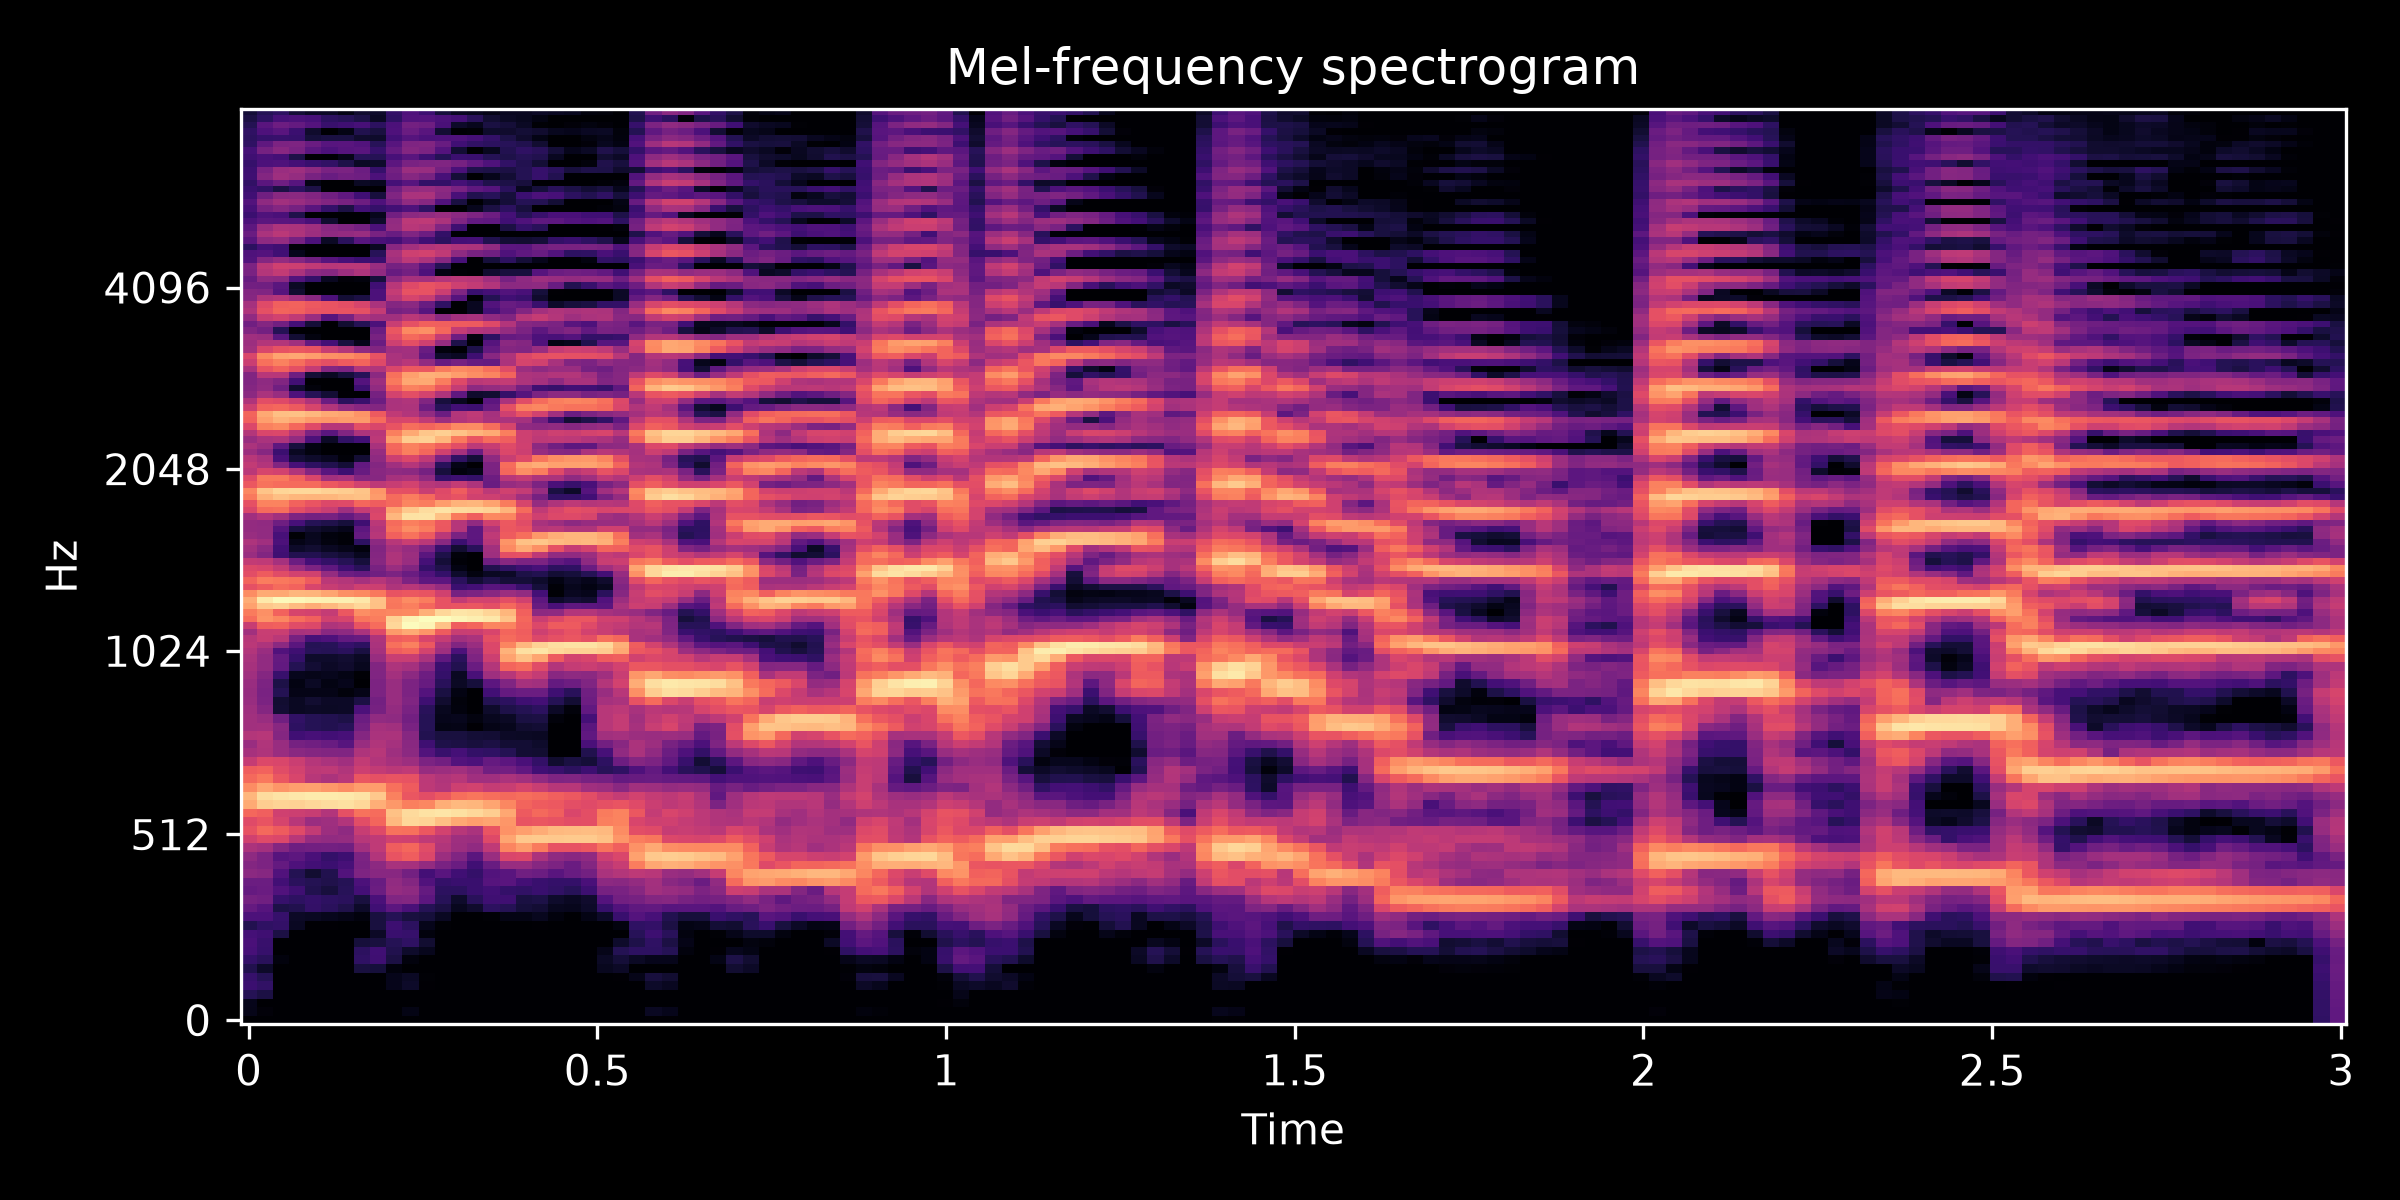
\includegraphics[width=1.0\textwidth]{images/img_dsp_spectrogram.png}
      \vspace{0.1cm}
      
\begin{lstlisting}
pre_emp = np.append(y[0], y[1:] - 0.97 * y[:-1])
frames = librosa.util.frame(
    pre_emp, frame_length=1024, hop_length=512).T
window = np.hamming(1024)
\end{lstlisting}
    \end{column}
    \begin{column}{0.45\textwidth}
      \textbf{Extracted Variables:}
      \begin{itemize}
          \item \texttt{y} (1D raw waveform)
          \item \texttt{pre\_emp} (High-pass filter boost)
          \item \texttt{frames} (Chunked audio blocks)
          \item \texttt{window} (Hamming taper)
          \item \texttt{S} (Mel-spectrogram magnitude)
          \item \texttt{mfcc} (Discrete Cosine Transform)
      \end{itemize}
    \end{column}
  \end{columns}
\end{frame}

% -----------------------------------------------------------------------------
\begin{frame}[fragile,t]{Emotion Identification (Non-Linear Dynamics)}
  \vspace{0.1cm}
  
  \begin{columns}[T,onlytextwidth]
    \begin{column}{0.53\textwidth}
      \centering
      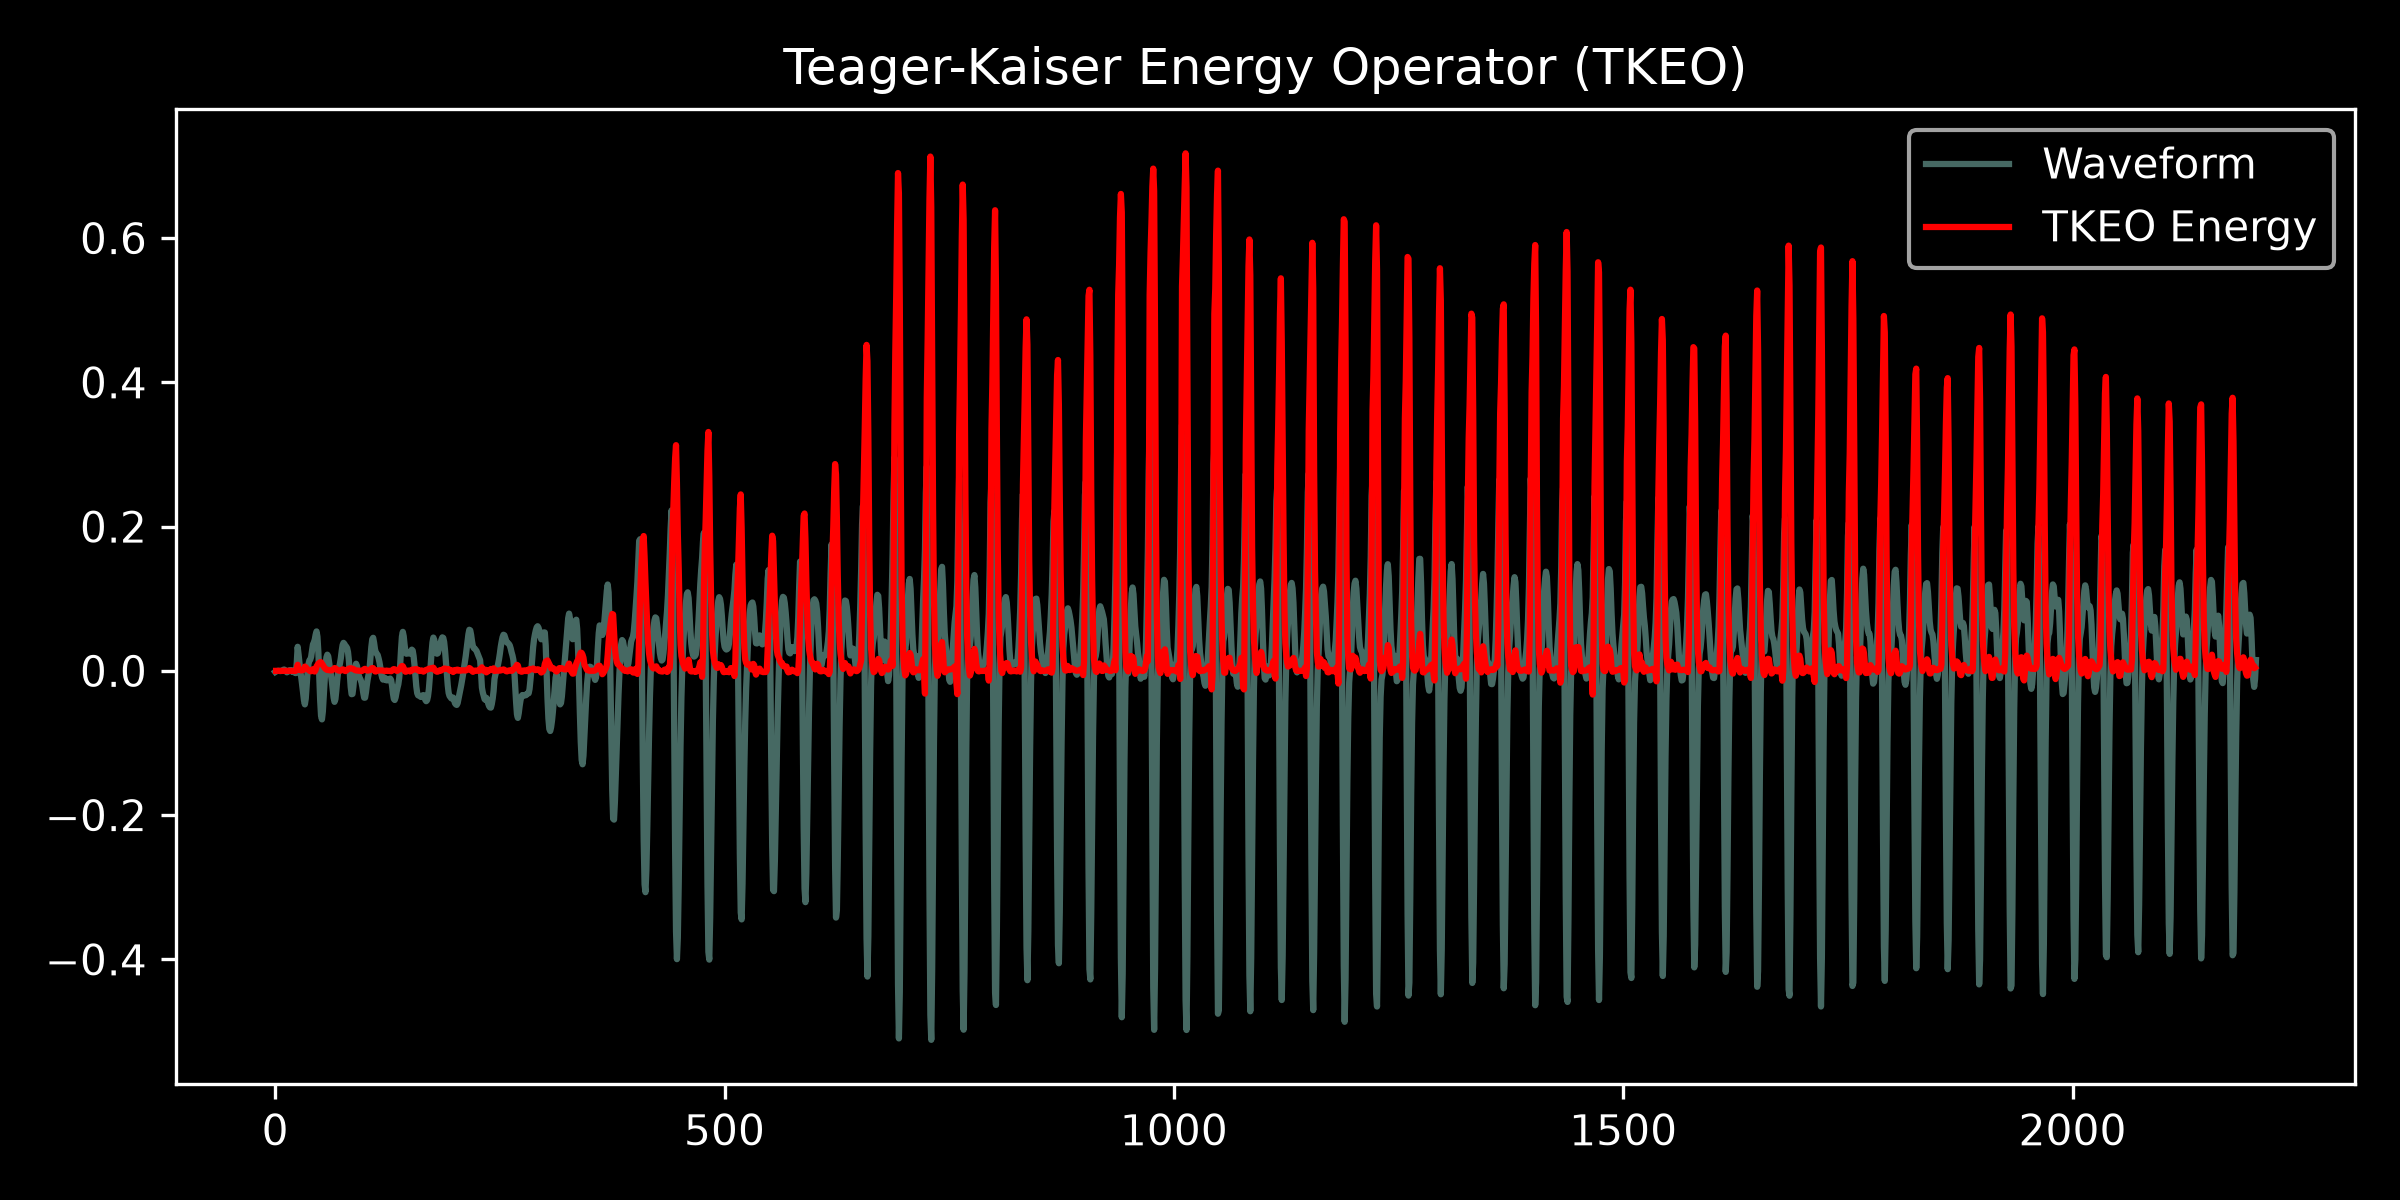
\includegraphics[width=1.0\textwidth]{images/img_emotion_tkeo.png}
      \vspace{0.1cm}
      
\begin{lstlisting}
tkeo = y[1:-1]**2 - y[:-2] * y[2:]
tkeo_val = float(np.mean(tkeo))
\end{lstlisting}
    \end{column}
    \begin{column}{0.45\textwidth}
      \textbf{Extracted Variables:}
      \begin{itemize}
          \item \texttt{mfcc\_mean} (Timbre signature)
          \item \texttt{mfcc\_std} (Timbre variance)
          \item \texttt{tkeo\_val} (Micro-tremor energy)
          \item \texttt{hnr\_val} (Harmonic-to-Noise clarity)
          \item \texttt{rolloff\_mean} (Spectral skewness)
          \item \texttt{zcr\_mean} (Zero-crossing rate)
          \item \texttt{onset\_mean, onset\_std} (Flux)
      \end{itemize}
    \end{column}
  \end{columns}
\end{frame}

% -----------------------------------------------------------------------------
\begin{frame}[fragile,t]{Language Identification (SDC Indexing)}
  \vspace{0.1cm}
  
  \begin{columns}[T,onlytextwidth]
    \begin{column}{0.53\textwidth}
      \centering
      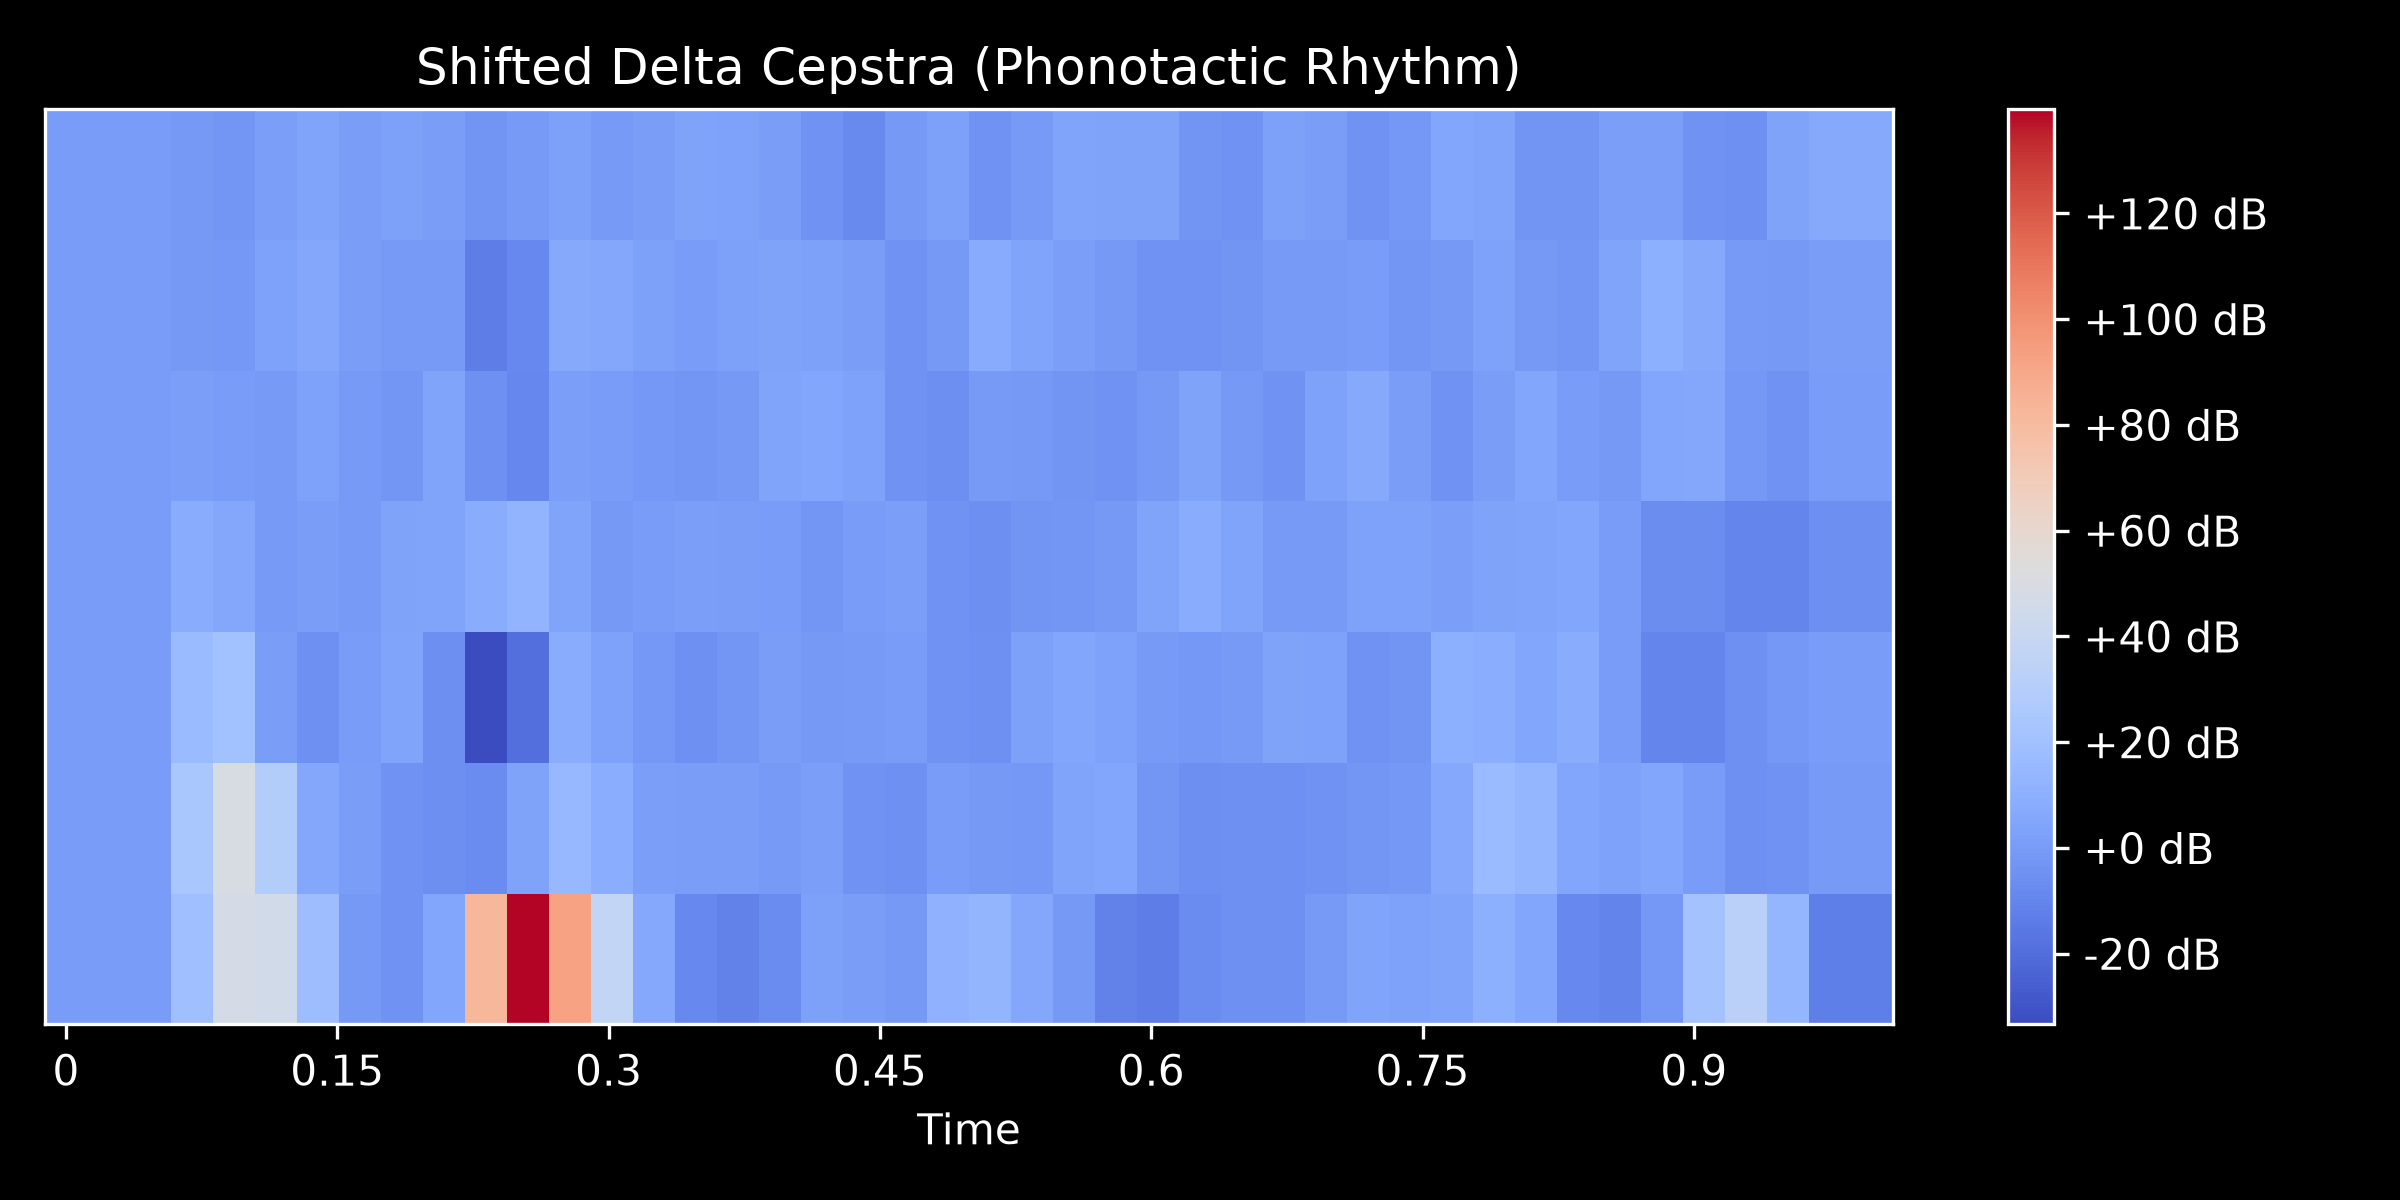
\includegraphics[width=0.9\textwidth]{images/img_language_sdc.png}
      \vspace{0.1cm}
      
\begin{lstlisting}
delta[:, t] = mfccs[:, right] - mfccs[:, left]
for t in range(valid_frames):
    sdc_frame = [delta[:, t + i*P] for i in range(k)]
\end{lstlisting}
    \end{column}
    \begin{column}{0.45\textwidth}
      \textbf{Extracted Variables:}
      \begin{itemize}
          \item \texttt{N=7} (MFCC base dimensions)
          \item \texttt{d=1} (Frame shift for delta)
          \item \texttt{P=3} (Gap between delta blocks)
          \item \texttt{k=7} (Concatenated blocks)
          \item \texttt{delta} (Temporal derivatives)
          \item \texttt{sdc\_frame} (49-Dim phonotactic rhythm)
          \item \texttt{valid\_frames} (Shiftable bounds)
      \end{itemize}
    \end{column}
  \end{columns}
\end{frame}

% -----------------------------------------------------------------------------
\begin{frame}[fragile,t]{Speaker Diarization (Spectral Graph Theory)}
  \vspace{0.1cm}
  
  \begin{columns}[T,onlytextwidth]
    \begin{column}{0.53\textwidth}
      \centering
      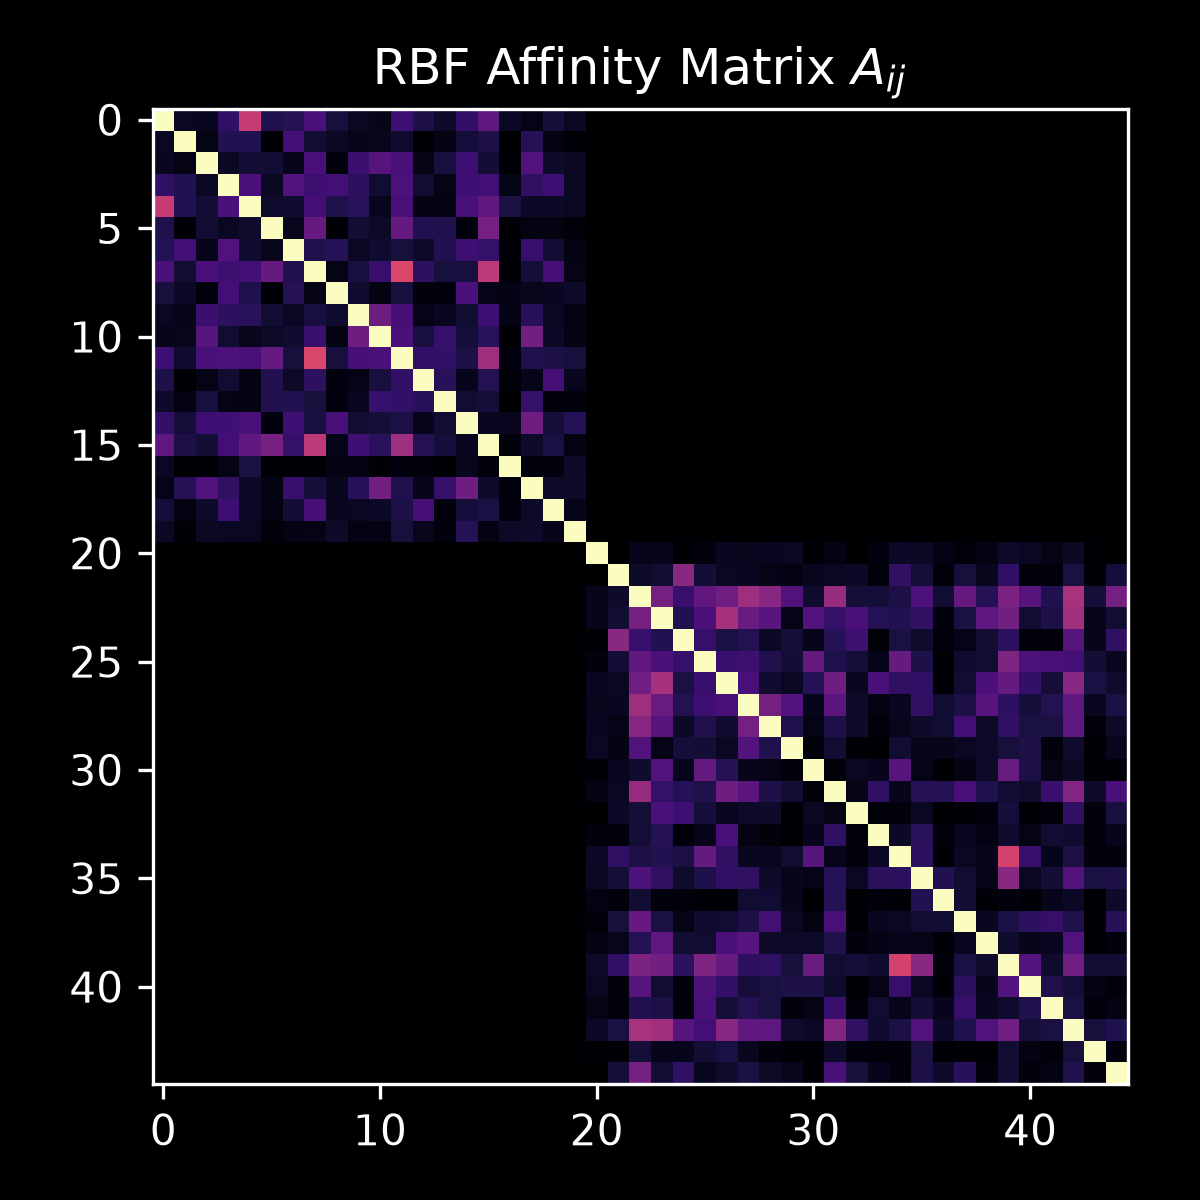
\includegraphics[width=0.7\textwidth]{images/img_diarization_graph.png}
      \vspace{0.1cm}
      
\begin{lstlisting}
pairwise_dists = squareform(pdist(X, 'euclidean'))
affinity_matrix = np.exp(-gamma * (pairwise_dists**2))
eigenvalues, eigenvectors = np.linalg.eigh(laplacian)
\end{lstlisting}
    \end{column}
    \begin{column}{0.45\textwidth}
      \textbf{Extracted Variables:}
      \begin{itemize}
          \item \texttt{non\_mute} (VAD active frames)
          \item \texttt{X} (Aggregated MFCC segments)
          \item \texttt{pairwise\_dists} (Euclidean space)
          \item \texttt{gamma} (RBF kernel bandwidth)
          \item \texttt{affinity\_matrix} ($A_{ij}$ connections)
          \item \texttt{laplacian} ($L_{sym}$ normalized graph)
          \item \texttt{eigenvectors[:, :2]} (Fiedler vector)
      \end{itemize}
    \end{column}
  \end{columns}
\end{frame}

% -----------------------------------------------------------------------------
\begin{frame}[fragile,t]{Transcription (Levinson-Durbin \& DTW)}
  \vspace{0.1cm}

  \begin{columns}[T,onlytextwidth]
    \begin{column}{0.53\textwidth}
      \centering
      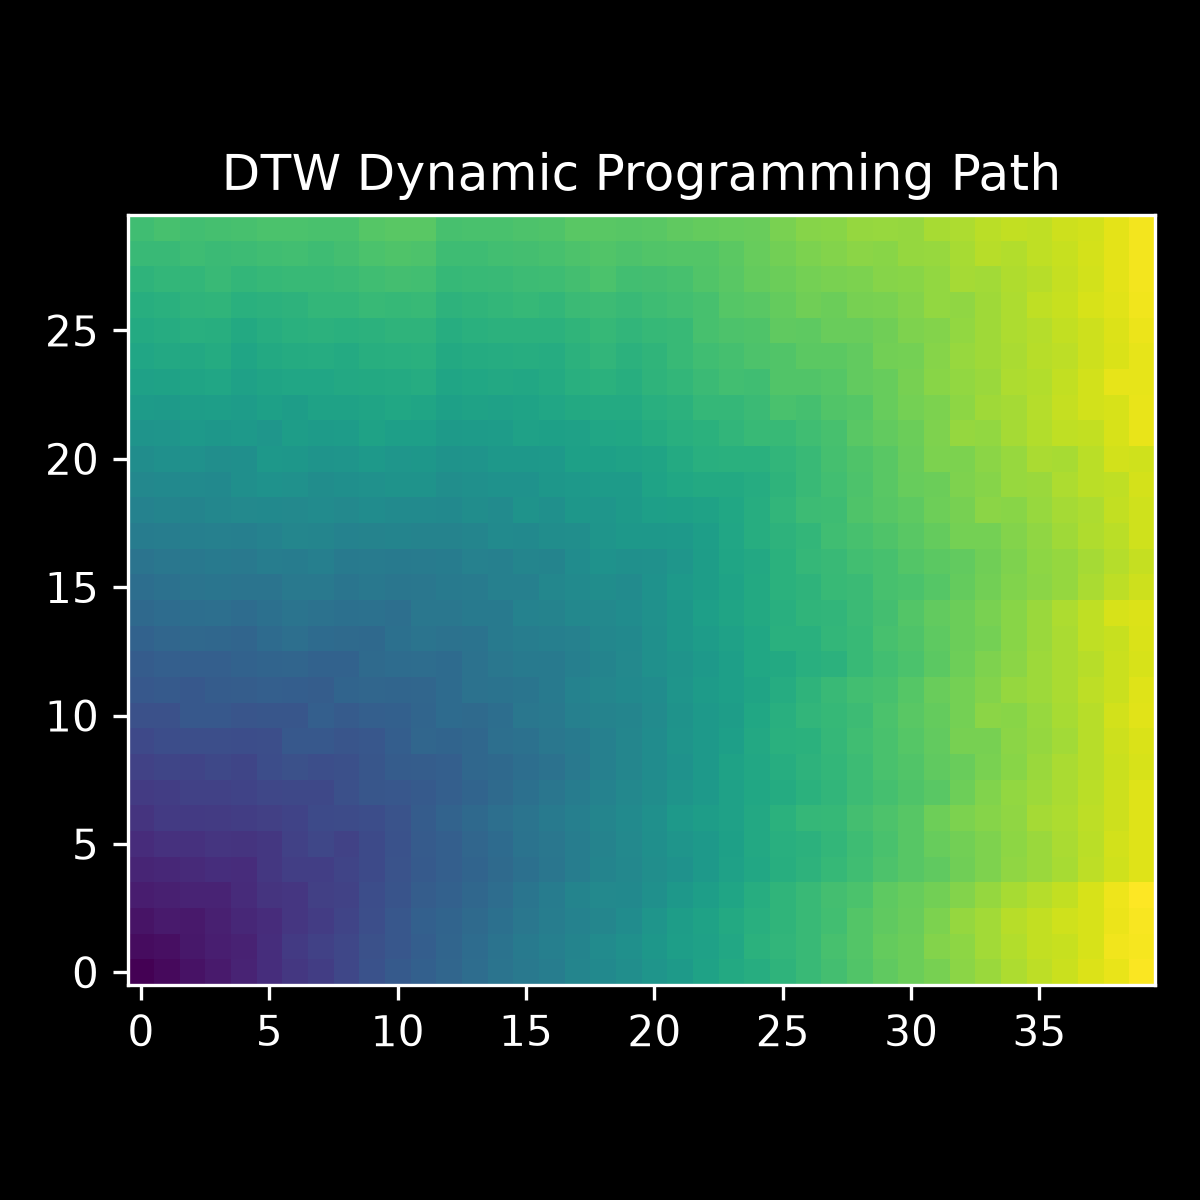
\includegraphics[width=0.7\textwidth]{images/img_transcription_dtw.png}
      \vspace{0.1cm}
      
\begin{lstlisting}
cost[i, j] = dist_mat[i-1, j-1] + min(
    cost[i-1, j], cost[i, j-1], cost[i-1, j-1])
\end{lstlisting}
    \end{column}
    \begin{column}{0.45\textwidth}
      \textbf{Extracted Variables:}
      \begin{itemize}
          \item \texttt{r} (Autocorrelation lags)
          \item \texttt{a\_k} (Levinson-Durbin coefficients)
          \item \texttt{segment\_lpcs} (Vocal tract shapes)
          \item \texttt{dist\_mat} (Euclidean frame distances)
          \item \texttt{cost} (DTW Dynamic Programming matrix)
          \item \texttt{min\_dist} (Normalized path distance)
          \item \texttt{matches\_found} (Subsequence NMS)
      \end{itemize}
    \end{column}
  \end{columns}
\end{frame}

% -----------------------------------------------------------------------------
\begin{frame}[fragile,t]{Audio Matching (Shazam Constellation Hashing)}
  \vspace{0.1cm}
  
  \begin{columns}[T,onlytextwidth]
    \begin{column}{0.53\textwidth}
      \centering
      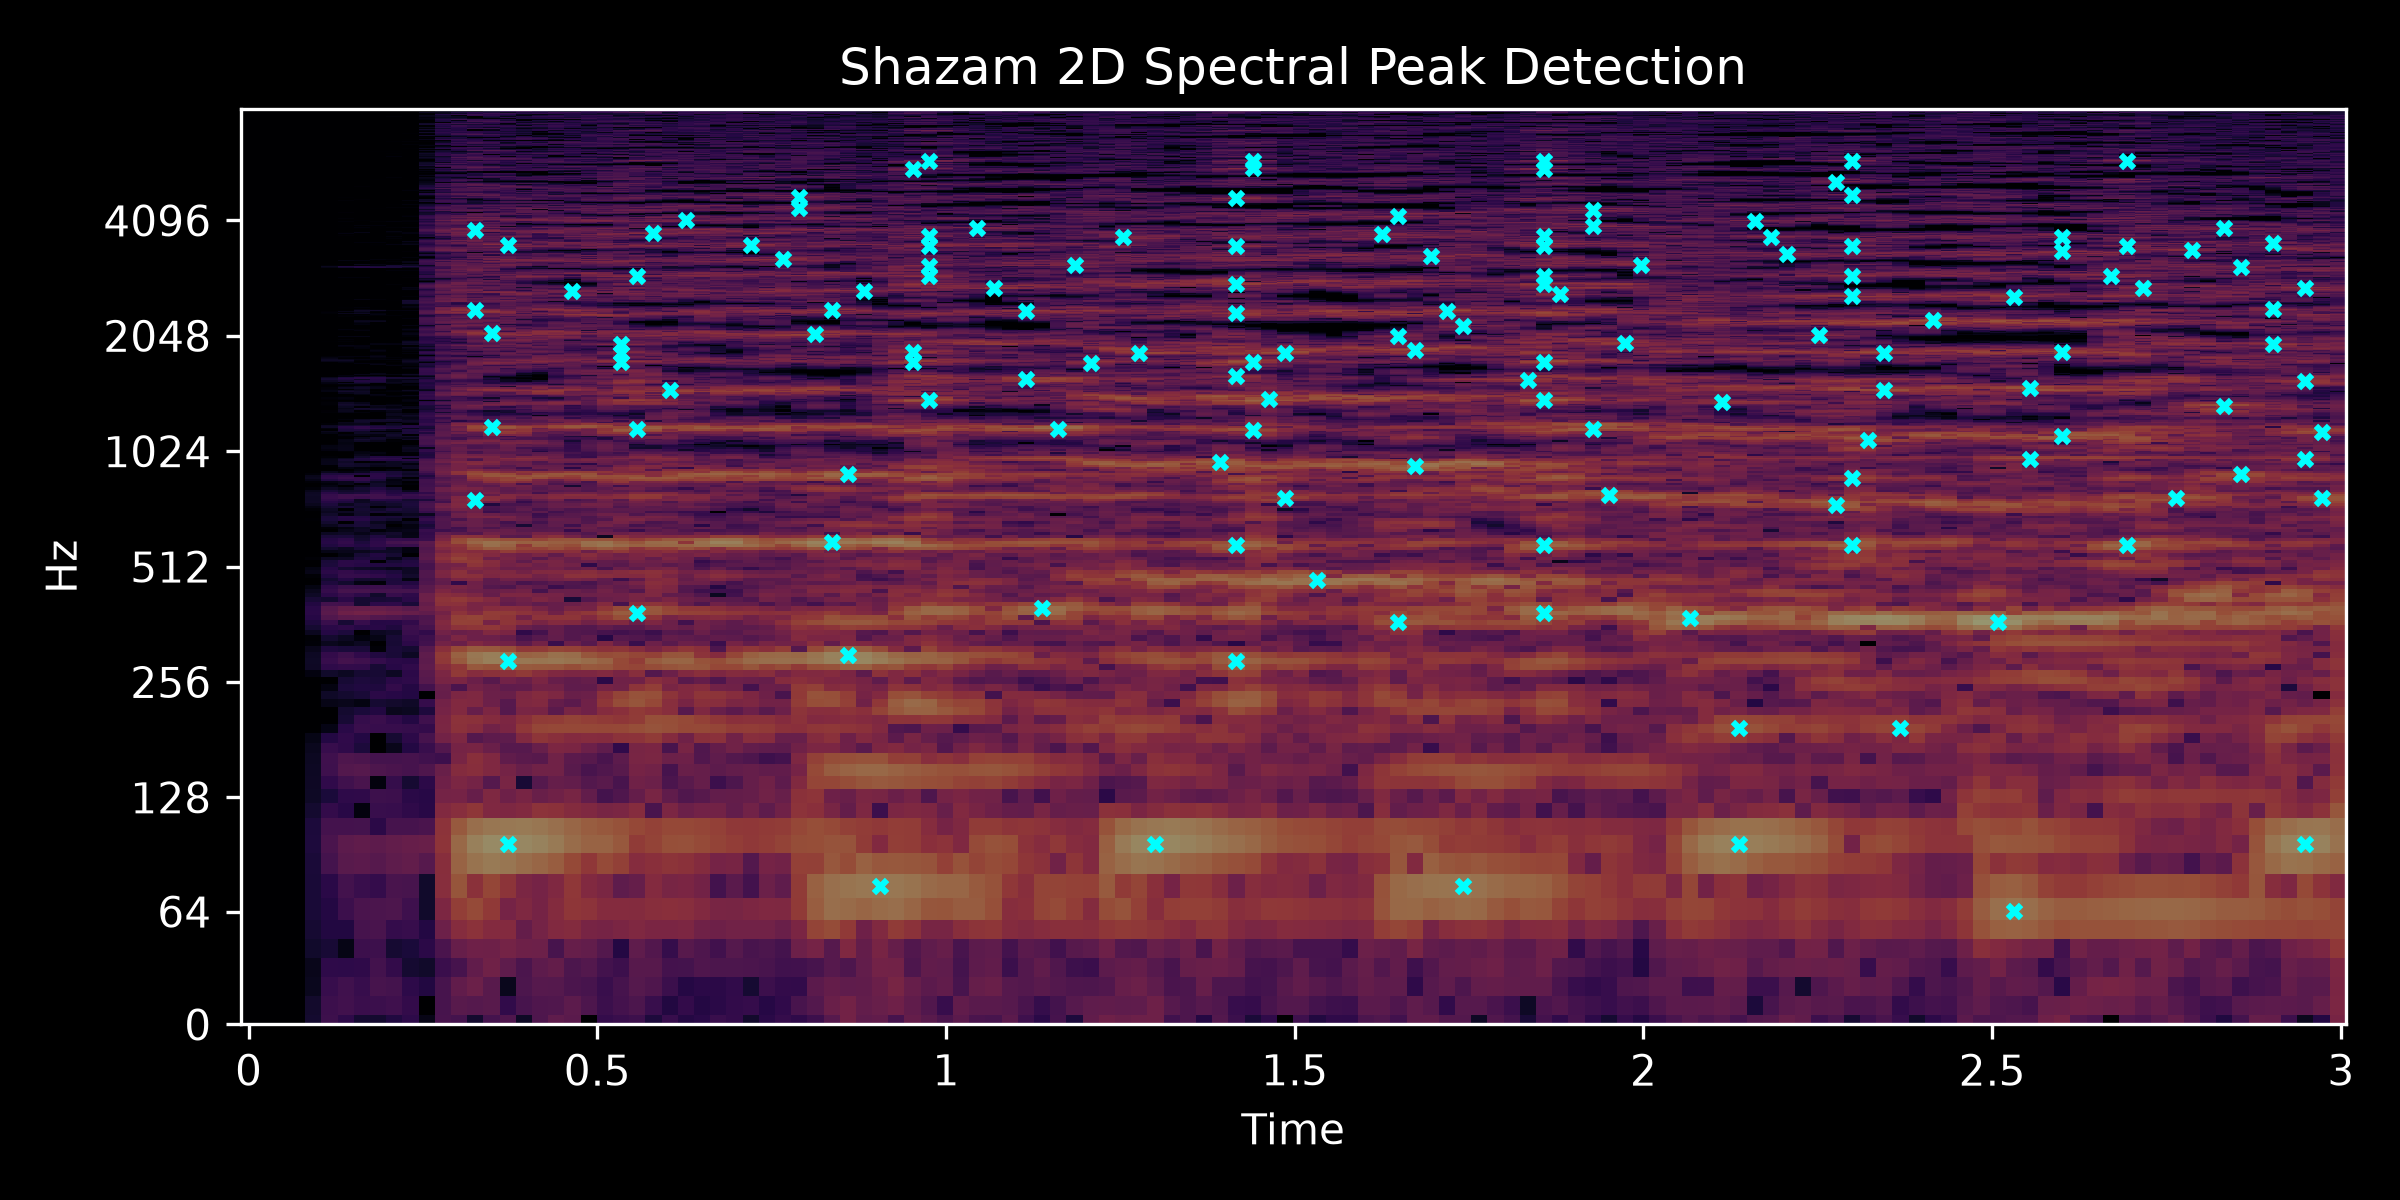
\includegraphics[width=1.0\textwidth]{images/img_music_constellation.png}
      \vspace{0.1cm}
      
\begin{lstlisting}
local_max = maximum_filter(
    magnitude, size=15) == magnitude
peaks_mask = local_max & (magnitude > threshold)
\end{lstlisting}
    \end{column}
    \begin{column}{0.45\textwidth}
      \textbf{Extracted Variables:}
      \begin{itemize}
          \item \texttt{magnitude} (STFT absolute values)
          \item \texttt{local\_max} (2D maximum filter peaks)
          \item \texttt{peaks\_mask} (Energy thresholded peaks)
          \item \texttt{f1, f2} (Paired peak frequencies)
          \item \texttt{delta\_t} (Time offset between peaks)
          \item \texttt{hash\_str} (Combinatorial geometry key)
          \item \texttt{tally} (Hough Transform histogram counts)
      \end{itemize}
    \end{column}
  \end{columns}
\end{frame}

% -----------------------------------------------------------------------------
\begin{frame}[fragile,t]{Evaluation \& Conclusion}
  \vspace{0.3cm}
  
  \textbf{Large-Scale System Evaluation (55 Unseen Audio Tracks):}
  \vspace{0.2cm}
  \begin{itemize}
      \item \textbf{Song Retrieval (Shazam): 100\% Accuracy}
      \begin{itemize}
          \item \textit{Why?} Geometric constellation hashes are mathematically immune to heavy white noise and cropping.
      \end{itemize}
      \item \textbf{Language Identification (SDC): 85.7\% Accuracy}
      \begin{itemize}
          \item \textit{Why?} Languages possess strict physical rhythm constraints that map perfectly to metric spaces.
      \end{itemize}
      \item \textbf{Emotion Identification: 37.0\% Accuracy}
      \begin{itemize}
          \item \textit{Why?} \textcolor{red}{The limit of classical DSP.} "Happy" and "Angry" share identical kinetic energy (TKEO) signatures. Without the semantic context of a Neural Network, math cannot differentiate subjective psychology.
      \end{itemize}
  \end{itemize}
\end{frame}

\end{document}
